\experiment{Shell Progrramming}{04/10/2023}

\section{Aim}
To write and execute basic shell programs.

\section{Files to Uppercase}

\subsection{Aim}
Accept one or more file names as arguments and convert the file contents to uppercase, provided they exist in the current directory.

\subsection{Algorithm}
\begin{enumerate}
   \item Start
   \item Read file name from command line
   \item For each file, convert the contents to uppercase
   \item Stop
\end{enumerate}

\subsection{Program}
\begin{lstlisting}[label={list:program:uppercase}]
for name in $@
do
   echo "file name:"$name
   tr '[:lower:]' '[:upper:]' < $name
   echo " "
done
\end{lstlisting}

\subsection{Sample Input and Output}
 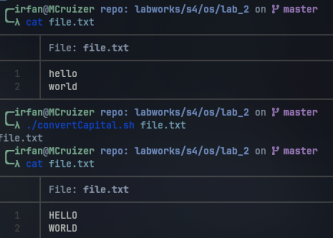
\includegraphics[]{Cycle_1//Outputs/ucase.png}

\section{Reversing Arguments}

\subsection{Aim}
Accept any number of arguments and print them in the reverse order.

\subsection{Algorithm}
\begin{enumerate}
   \item Start
   \item Read the arguments and store in an array
   \item Print the array in reverse order
   \item Stop
\end{enumerate}

\subsection{Program}
\begin{lstlisting}[label={list:program:reverse_args}]
a=("$@")
n=$#
for(( i=$n-1; i>=0; i-- ))
do
   echo "${a[$i]}"
done
\end{lstlisting}

\subsection{Sample Input and Output}
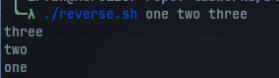
\includegraphics[]{Cycle_1//Outputs/revers.png}

\section{Gross Salary Calculation}

\subsection{Aim}
Compute the gross salary of an employee according to the following rules:
\begin{itemize}
   \item If the basic salary is less than 1500, then HRA = 10\% of the basic and DA = 90\% of the basic.
   \item If the basic salary is greater than or equal to 1500, then HRA = Rs. 500 and DA = 98\% of the basic.
\end{itemize}

\subsection{Algorithm}
\begin{enumerate}
   \item Start
   \item Read basicSalary
   \item If basicSalary < 1500, then HRA = (0.1) * basicSalary and DA = (0.9) * basicSalary
   \item Else HRA = 500 and DA = (98/100) * basicSalary
   \item Print HRA and DA
   \item Stop
\end{enumerate}

\subsection{Program}
\begin{lstlisting}[label={list:program:gross_salary}]
read -p "Basic pay:" basic

if [ $basic -lt 1500 ]
then
   hra=$(echo "$basic * 0.1" | bc)
   da=$(echo "$basic * 0.9" | bc)
else
   hra=500
   da=$(echo "$basic * 0.98" | bc)
fi

gross=$(echo "$basic + $hra + $da" | bc)
echo "Gross Salary: Rs. $gross"
\end{lstlisting}

\subsection{Sample Input and Output}
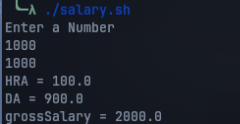
\includegraphics[]{Cycle_1//Outputs/salary.png}

\section{Smallest of Three Numbers}

\subsection{Aim}
Find the smallest of three numbers that are read from the keyboard.

\subsection{Algorithm}
\begin{enumerate}
   \item Start
   \item Read a, b, c
   \item If a < b and a < c, then print a
   \item Else if b < a and b < c, then print b
   \item Else print c
   \item Stop
\end{enumerate}

\subsection{Program}
\begin{lstlisting}[label={list:program:smallest_three}]
read -p "Enter 1st number " num1
read -p "Enter 2nd number " num2
read -p "Enter 3rd number " num3

if [ $num1 -lt $num2 ] && [ $num1 -lt $num3 ]
then
   smallest=$num1
elif [ $num2 -lt $num1 ] && [ $num2 -lt $num3 ]
then
   smallest=$num2
else
   smallest=$num3
fi

echo "The smallest number is: $smallest"
\end{lstlisting}

\subsection{Sample Input and Output}
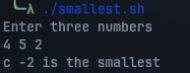
\includegraphics[]{Cycle_1//Outputs/smallest.png}

\section{Reversing Number}

\subsection{Aim}
Print a number in reverse order.

\subsection{Algorithm}
\begin{enumerate}
   \item Start
   \item Enter the number n
   \item while n > 0, do steps 4 and 5
       \begin{enumerate}
           \item r = r * 10 + n \% 10
           \item n = n / 10
       \end{enumerate}
   \item print r
   \item Stop
\end{enumerate}

\subsection{Program}
\begin{lstlisting}[label={list:program:reverse_number}]
read -p "Enter number" n
r=0
while [ $n -gt 0 ] ; do
   r=$((r*10+n%10))
   n=$((n/10))
done
echo $r
\end{lstlisting}

\subsection{Sample Input and Output}
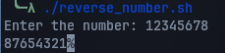
\includegraphics[]{Cycle_1//Outputs/revess.png}


\section{Armstrong Numbers}

\subsection{Aim}
Print all Armstrong numbers between two given numbers.

\subsection{Algorithm}
\begin{enumerate}
   \item Start
   \item Input $n1$ and $n2$
   \item $i = n1$
   \item While $i \leq n2$, repeat steps 5 to 12
       \begin{enumerate}
           \item $a = i$
           \item $s = 0$
           \item $l = \text{length}(i)$
           \item While $a > 0$, repeat steps 8 to 10
               \begin{enumerate}
                   \item $k = a \, \% \, 10$
                   \item $s = s + k^l$
                   \item $a = \lfloor a / 10 \rfloor$
               \end{enumerate}
           \item If $s = i$, print $i$
       \end{enumerate}
   \item Increment $i$
   \item Stop
\end{enumerate}


\subsection{Program}
\begin{lstlisting}[label={list:program:armstrong_numbers}]
read -p "Enter number 1 :" n1
read -p "Enter number 2 :" n2

for (( i=$n1 ; i<=$n2 ; i++ ))
do
   s=0
   a=$i
   l=${#a}
   while [ $a -gt 0 ]
   do
       k=$((a%10))
       s=$((k**l+s))
       a=$((a/10))
   done
   if [ $s -eq $i ]
   then
       echo $i
   fi
done
\end{lstlisting}

\subsection{Sample Input and Output}
 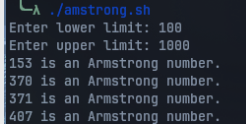
\includegraphics[]{Cycle_1//Outputs/amstrong.png}


\section{Number Pattern}

\subsection{Aim}
Print the following pattern up to n rows, for a given n:
\begin{verbatim}
1
2 2
3 3 3
4 4 4 4
.
.
n n n n n ..
\end{verbatim}

\subsection{Algorithm}
\begin{enumerate}
   \item Start
   \item Read n
   \item i = 1
   \item While i <= n, repeat steps 5 to 10
       \begin{enumerate}
           \item j = 0
           \item While j < i, repeat steps 7 and 8
               \begin{enumerate}
                   \item Print i
                   \item Increment j
               \end{enumerate}
           \item Print newline
           \item Increment i
       \end{enumerate}
   \item Stop
\end{enumerate}

\subsection{Program}
\begin{lstlisting}[label={list:program:number_pattern}]
read -p "Enter n" n

for (( i=1; i<=n; i++ ))
do
   for (( j=0; j<i; j++ ))
   do
       echo -n $i
   done
   echo ""
done
\end{lstlisting}

\subsection{Sample Input and Output}
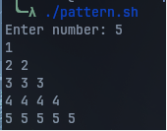
\includegraphics[]{Cycle_1//Outputs/patern.png}

\section{Password Validation}

\subsection{Aim}
Validate password strength. The password string should meet the following assumptions:
\begin{itemize}
   \item Length should be a minimum of 8 characters.
   \item Should contain both small and capital case letters, at least one digit, and an underscore.
\end{itemize}
If the password doesn't comply with any of the above conditions, then the script should report it as a Weak Password.

\subsection{Algorithm}
\begin{enumerate}
   \item Start
   \item Read password
   \item If the length of the password is greater than 8 and the password contains at least one uppercase letter, one lowercase letter, one digit, and an underscore, then print "Strong password"
   \item Else print "Weak password"
   \item Stop
\end{enumerate}

\subsection{Program}
\begin{lstlisting}[label={list:program:password_validation}]
read -p "Enter your password: " password

if [ ${#password} -ge 8 ] && [[ $password =~ [a-z] ]] &&
  [[ $password =~ [A-Z] ]] && [[ $password =~ [0-9] ]] && [[ $password =~ [_] ]];
then
   echo "Strong Password"
else
   echo "Weak Password"
fi
\end{lstlisting}

\subsection{Sample Input and Output}
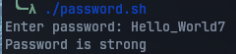
\includegraphics[]{Cycle_1//Outputs/password.png}


\section{Binary and Hexadecimal}

\subsection{Aim}
Print the binary and hexadecimal equivalent of a decimal number.

\subsection{Algorithm}
\begin{enumerate}
   \item Start
   \item Read Decimal number
   \item Initialize b=d, i=0, a[]
   \item while(d > 0) do steps 5 to 7
       \begin{enumerate}
           \item a[i] = d \% 2
           \item d = d / 2
           \item i = i + 1
       \end{enumerate}
   \item print a from index i-1 to 0
   \item set i = 0, d = b, a[]
   \item while(d > 0) do steps 10 to 14
       \begin{enumerate}
           \item r = d \% 16
           \item if (r < 10) then a[i] = r
           \item else
               \begin{enumerate}
                   \item if r = 10, a[i] = "A"
                   \item if r = 11, a[i] = "B"
                   \item if r = 12, a[i] = "C"
                   \item if r = 13, a[i] = "D"
                   \item if r = 14, a[i] = "E"
                   \item if r = 15, a[i] = "F"
               \end{enumerate}
           \item d = d / 16
           \item i = i + 1
       \end{enumerate}
   \item print a from index i-1 to 0
   \item Stop
\end{enumerate}

\subsection{Program}
\begin{lstlisting}[label={list:program:binary_hex}]
read -p "Enter decimal number" d

a=()
b=$d
i=0

while [ $d -gt 0 ]
do
   a[i]=$((d%2))
   d=$((d/2))
   i=$((i+1))
done

echo -n "Binary of $b is "
for (( j=$i-1; j>=0; j-- ))
do
   echo -n "${a[$j]}"
done
echo ""

a=()
i=0
d=$b
while [ $d -gt 0 ]
do
   r=$((d%16))
   if [ $r -lt 10 ]
   then
       a[i]=$r
   else
       case $r in
           10) a[i]="A";;
           11) a[i]="B";;
           12) a[i]="C";;
           13) a[i]="D";;
           14) a[i]="E";;
           15) a[i]="F";;
       esac
   fi
   d=$((d/16))
   i=$((i+1))
done

echo -n "Hexadecimal of $b is "
for (( j=$i-1; j>=0; j-- ))
do
   echo -n "${a[$j]}"
done
echo ""
\end{lstlisting}

\subsection{Sample Input and Output}
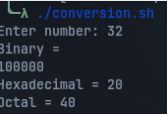
\includegraphics[]{Cycle_1//Outputs/conversions.png}

\section{3 Digit Numbers}
\subsection{Aim}
Generate all 3 digit numbers that contain only the digits 0, 1, 2, 3 (number does not start with 0).

\subsection{Algorithm}
\begin{enumerate}
   \item Start
   \item for i=1 to i=3 do steps 3 and 4
   \item for j=0 to j=3 do step 4
   \item for k=0 to k=3 print (ijk)
   \item Stop
\end{enumerate}

\subsection{Program}
\begin{lstlisting}[label={list:c_program:queue}]
for (( i=1; i<=3; i++ ))
do
    for (( j=0; j<=3; j++ ))
    do
        for(( k=0; k<=3; k++ ))
        do
            echo $i$j$k
            c=$((c+1))
        done
    done
done
\end{lstlisting}

\subsection{Sample Input and Output}
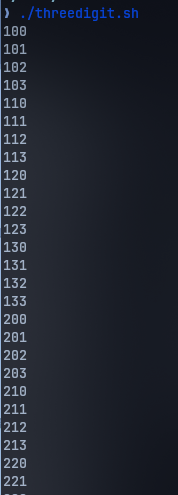
\includegraphics[]{Cycle_1//Outputs/threegiti.png}


\section{Summarize Directory}
\subsection{Aim}
Create the command 'summarize directory' which takes a directory as input and summarizes the contents in the directory. This command has to print the a. Total Number of Files in the directory b. List of all extensions of files present c. Count of files having each extension in new lines The command works recursively for all the subdirectories.

\subsection{Algorithm}
\begin{enumerate}
   \item Start
   \item Read path from terminal
   \item if directory does not exist, print directory not found and stop
   \item if number of arguments is 0, print Usage: Summarize\_directory and stop
   \item Find the number of files and print it.
   \item Iterate through all files and store its extensions and print it.
   \item Extract unique extensions and find count of each and print it.
   \item for all subdirectories repeat steps 5 to 7.
   \item Stop
\end{enumerate}

\subsection{Program}
\begin{lstlisting}[label={list:c_program:queue}]
summarize_dir() {
    dir="$1"
    file_ext=""
    count=0
    num_files=$(find "$dir" -type f | wc -l)
    echo "Total Number of Files in the Directory: $num_files"
    for file in $(find "$dir" -type f); do
        file_ext=$(echo "${file##*.}")
        echo "$file_ext"
    done | sort -u > extensions.txt
    
    while read ext; do
        count=$(find "$dir" -type f -name "*.$ext" | wc -l)
        echo "$ext: $count"
    done < extensions.txt
    rm extensions.txt
}
if [ -z "$1" ]; then
    echo "Usage: summarize_directory [directory]"
    exit 1
fi
if [ ! -d "$1" ]; then
    echo "Error: Directory does not exist."
    exit 1
fi
for subdir in $(find "$1" -type d); do
    summarize_dir "$subdir"
done
\end{lstlisting}

\subsection{Sample Input and Output}
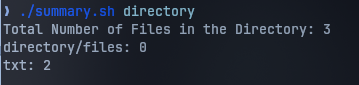
\includegraphics[width=0.5\linewidth]{Cycle_1//Outputs/summary.png}

\section{Pass/Fail}

\subsection{Aim}
Given a file containing the marks obtained by students for 3 subjects in an exam. In order to pass, a student should score at least 50 marks in every subject. The file has one record (line) for each student in the following format: rollnum-ber subject1 subject2 subject3 Write a script to print pass/ fail status of each student in the following format: rollnumber pass/fail.

\subsection{Algorithm}
\begin{enumerate}
   \item Start
   \item Read File name
   \item For each line in the file do steps 4 and 5
   \item If all 3 marks are greater than or equal to 50, set status="Pass" else set status="fail".
   \item Print (rollno, status)
   \item Stop
\end{enumerate}

\subsection{Program}
\begin{lstlisting}[label={list:program:pass_fail}]
read -p "Enter the file name: " file

while read line
do
   echo "$line"
   fields=($line)
   roll=${fields[0]}
   sub1=${fields[1]}
   sub2=${fields[2]}
   sub3=${fields[3]}

   if (( sub1 >= 50 && sub2 >= 50 && sub3 >= 50 ))
   then
       status="pass"
   else
       status="fail"
   fi

   echo "$roll $status"
done < $file
\end{lstlisting}

\subsection{Sample Input and Output}
 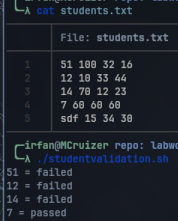
\includegraphics[]{Cycle_1//Outputs/passorfial.png}

\section{Palindromic Prime}
\subsection{Aim}
Find the smallest prime number greater than \( n \) which is palindromic.

\subsection{Algorithm}
\begin{enumerate}
    \item Start
    \item Read \( n \)
    \item Initialize \( f = 0 \)
    \item while (\( f == 0 \)) do steps
    \item \( n = n + 1 \)
    \item for \( i = 2 \) to \( \text{squareroot}(n) \)
    \item if \( n \mod i = 0 \) set \( f = 1 \) and break
    \item if \( f = 0 \) then
    \item set \( r = 0, num = n \)
    \item while (\( num > 0 \)) do
    \item \( r = r \times 10 + \text{num} \mod 10 \)
    \item \( \text{num} = \text{num} / 10 \)
    \item if \( r = n \) then
    \item set \( f = 1 \)
    \item print \( n \)
    \item else
    \item set \( f = 0 \)
    \item else set \( f = 0 \)
    \item Stop
\end{enumerate}
\subsection{Program}

\begin{lstlisting}[label={list:program:palindromic_prime}
read -p "Enter n" n
f=0
while [ $f -eq 0 ]
do
    n=$((n+1))
    for (( i=2; i*i<=n; i++ ))
    do
        if [ $((n%i)) -eq 0 ]
        then
            f=1
            break
        fi
    done
    if [ $f -eq 0 ]
    then
        r=0
        num=$n
        while [ $num -gt 0 ]
        do
            r=$((r*10+num%10))
            num=$((num/10))
        done
        if [ $r -eq $n ]
        then
            f=1
            echo "The next palindromic prime number is $n"
        else
            f=0
        fi
    else
        f=0
    fi
done
\end{lstlisting}
\subsection{Sample Input and Output}
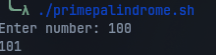
\includegraphics[]{Cycle_1//Outputs/pandrimicprime.png}

\section{Pattern}
\subsection{Aim}
Shell program to print the following pattern up to \( n \) rows, for a given \( n \):
\[
\begin{array}{cccc}
* & & & \\
* & * & * & \\
* & * & * & * \\
* & * & * & \\
* & & & \\
\end{array}
\]

\subsection{Algorithm}
\begin{enumerate}
    \item Start
    \item Read \( n \)
    \item if \( n \) is even set \( r = \frac{n}{2} \) else set \( r = \frac{n}{2} + 1 \)
    \item Initialize \( c = 0 \)
    \item for \( i = 1 \) to \( n \) do steps 6 to 12
    \item Set \( j = 1 \)
    \item while (\( j \leq r - c - 1 \)) do
    \item print " "
    \item \( j = j + 1 \)
    \item while (\( j \leq r + c \)) do
    \item print "*"
    \item \( j = j + 1 \)
    \item if (\( i < r \)) then Increment \( c \)
    \item if (\( i = r \) and \( n \) is odd) then Decrement \( c \)
    \item Else Decrement \( c \)
    \item Print newline
    \item Stop
\end{enumerate}

\subsection{Program}
\begin{lstlisting}[label={list:program:pass_fail}]
#!/bin/bash
read -p "Enter number: " n

for (( i = 1; i <= n; i++ )); do
	for (( j = 0; j < i*2-1 ; j++ )); do
		echo -ne "* "
	done
	echo ""
done
for (( i = n-1; i >= 1; i-- )); do
	for (( j = 0; j < i*2-1 ; j++ )); do
		echo -ne "* "
	done
	echo ""
done
\end{lstlisting}
\subsection{Sample Input and Output}
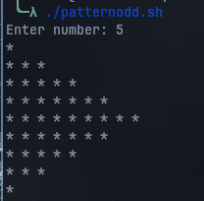
\includegraphics[]{Cycle_1//Outputs/pattrn.png}

\section{Result}
Basic shell programs were written and executed successfully.